\documentclass[lualatex]{ipsj}
% \documentclass[uplatex,dvipdfmx]{ipsj}

%------------------------------------------------------------------------------%
% Import your preferred packages
%------------------------------------------------------------------------------%

% Graphics (figures and colors)
\usepackage{graphicx,xcolor}

% \usepackage{fontenc}
\usepackage[T1]{fontenc}
\usepackage{lmodern}

% Mathematics markup
\usepackage{latexsym,amsmath}
\usepackage[all, warning]{onlyamsmath}% Warn the use of non-ams­math math­e­mat­icc

% Writing algorithms
\usepackage[linesnumbered,plain,vlined,figure]{algorithm2e}

% Using smart tables
\usepackage{booktabs,multirow}
\setlength\heavyrulewidth{0.4mm}
\setlength\lightrulewidth{0.1mm}
\setlength\cmidrulewidth{0.1mm}

% Using smart citations
\usepackage{cite,url}

% Using smart alphabets
\usepackage{newtxtext,newtxmath}

%------------------------------------------------------------------------------%
% Define your macros
%------------------------------------------------------------------------------%
% For definition and theorem environments
\newtheorem{definition}{定義}
\newtheorem{theorem}{定理}
\newtheorem{proof}{証明}
\renewcommand{\theproof}{}
\newcommand{\QED}{\hfill $\Box$}

% For references
\newcommand{\Sec}[1]{#1~章}
\newcommand{\Subsec}[1]{#1~節}
\newcommand{\Fig}[1]{図~#1}
\newcommand{\Tab}[1]{表~#1}
\newcommand{\Def}[1]{定義~#1}
\newcommand{\Theo}[1]{定理~#1}
\newcommand{\Eq}[1]{式~(#1)}

%------------------------------------------------------------------------------%
% Describe paper's title, authors, and authors' affiliations.
%------------------------------------------------------------------------------%
% \title
%   {<japanese_title>}
%   {<english_title>}
\title
  {全国大会及びFIT用クラスファイルの使い方}
  {How to use the class file for the national convention of IPSJ and FIT}
% \author
%   {<japanese_name>}
%   {<english_name>}
%   {<affiliation_label>[,<additional_affiliation>,...]}
\author{山田 太郎}{Tarou Yamada}{IE}
\author{山田 花子}{Hanako Yamada}{I}
\author{鈴木 太郎}{Tarou Suzuki}{I,IS}
% \affiliation{<affiliation_label>}
%   {<japanese_affiliation>}
%   {<english_affiliation>}
\affiliation{IE}
  {名古屋大学工学部電気電子・情報工学科}
  {Department of Information Engineering, School of Engineering, Nagoya University}
\affiliation{I}
  {名古屋大学大学院情報学研究科}
  {Graduate School of Informatics, Nagoya University}
\affiliation{IS}
  {名古屋大学大学院情報科学研究科}
  {Graduate School of Information Science, Nagoya University}

\begin{document}
\maketitle

%------------------------------------------------------------------------------%
% Describe your document
%------------------------------------------------------------------------------%
\section{はじめに}
本稿では,情報処理学会全国大会及びFITに投稿する論文用のクラスファイル``ipsj.cls''の使用法を説明する.
なお,本稿を作成するためのソースファイルは本クラスファイルのテンプレートも兼ねている.
つまり,コメントで``Describe ...''と書いてある箇所を変更することで,ソースファイルをそのまま論文作成に使用できる.


\section{使い方}
基本的な書き方は{\LaTeXe}で文章を書く際と同じであり,タイトル・著者・所属の指定方法のみ拡張している.
使用エンジンについてはBXjsclsを基に使用しており,upLaTeX及びLuaLaTeXでの動作確認を行った.
以下,エンジンの指定方法とタイトルなどの入力方法について説明する.

  \subsection{エンジンの指定}
  使用するエンジンはクラスのオプションとして指定する.
  例えば,LuaLaTeXを使用する場合は下記のようにオプションを指定する.
  \begin{quote}
    \texttt{\textbackslash documentclass[lualatex]\{ipsj\}}
  \end{quote}
  一方,upLaTeXを使用する場合は以下のように指定する.
  \begin{quote}
    \texttt{\textbackslash documentclass[uplatex,dvipdfmx]\{ipsj\}}
  \end{quote}

  なお,BXjscls自体は他のエンジンも使用できるが,このipsj.clsでは上記2エンジンのみを対象としている.
  もし他のエンジンを使用したい場合は,適宜クラスファイルを修正して使ってほしい.

  \subsection{タイトル・著者・所属の入力}
  タイトルを指定する際は,以下のように日本語タイトルを第1引数に,英語タイトルを第2引数に指定する.
    \begin{quote}
    \texttt{\textbackslash title}\{日本語タイトル\}\{english title\}
    \end{quote}

  著者を入力する際は,第1引数に日本語名を,第2引数に英語名を,第3引数に後述する所属ラベルを指定し,人数分列挙する.
    \begin{quote}
    \texttt{\textbackslash author}\{日本語名\}\{english name\}\{L\}
    \end{quote}
  所属が複数ある場合は,以下のように半角カンマ(,)区切りでラベルを列挙する.
    \begin{quote}
    \texttt{\textbackslash author}\{日本語名\}\{english name\}\{L1,L2\}
    \end{quote}

  所属を入力する際は,第1引数にラベルを,第2引数に日本語での所属を,第3引数に英語での所属名を指定する.
    \begin{quote}
    \texttt{\textbackslash affiliation}\{L\}\{日本語所属\}\{english affl.\}
    \end{quote}
  なお,``\texttt{\textbackslash author}''で使用したラベルが``\texttt{\textbackslash affiliation}''に存在しない場合,エラーが発生するため注意すること.

  また,著者と所属の表示順は,入力された順番にそのまま表示される.
  これは参照符についても同様であり,著者入力時のラベルで指定した順番に付与される.
  したがって,所属の出力順と参照符の付与順に関しては手動であわせる必要がある(自動化できるとは思いますが,面倒なのでたぶんやりません).


\section{出力例}
本章では,章節項や図表,アルゴリズムの出力例を示す.
なお,本クラスファイルは``bxjsarticle.cls''の拡張であり,各レイアウトは変更していないため,``bxjsarticle.cls''を用いた際と同様の出力結果が得られる(はずである).
したがって,章節項のレイアウトを変更したい場合は,``bxjsarticle.cls''での変更例を参考にすればよい.

  \subsection{節}
  節の出力例.

    \subsubsection{項}
    項の出力例.

      \paragraph{見出し付きパラグラフ}
      パラグラフの出力例.
  
  \subsection{図の出力例}
  図の出力例を\Fig{\ref{fig:sample}}に示す.
  
    \begin{figure}[t]
    \centering
    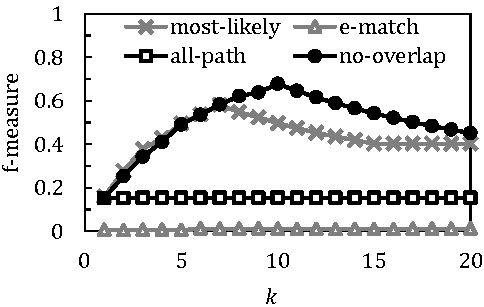
\includegraphics[scale=0.8]{./figures/sample_graph.pdf}
    \caption{図の例}
    \label{fig:sample}
    %\vspace{-5mm} % 文章とのスペースが気になるときは,適当に狭める
    \end{figure}
  
  以下,図を使用する際の注意点を列挙する.
  
    \paragraph{PDFファイルを使う:}
    以前は論文をDVIファイルで提出するのが主流だったため図もEPSファイルで作成していたが,現代ではほぼ間違いなくPDFファイルの提出を求められる.
    したがって,PowerPointなどで作成した図を直接PDFファイルとして保存し,挿入すればよい.
    
    ただし,PDFファイルを挿入する際は,画像のバウンディングボックスについての情報を持つXBBファイルを用意する必要がある.
    無い場合はコンパイル時に自動で用意されるが,数が多くなると時間がかかるため,あらかじめ``\texttt{extractbb}''コマンドで作成した方がよい.

    また,PowerPointでPDFファイルを作成した場合,ファイルの容量が無駄に大きくなるため,GhostScriptを用いて容量を削減することを勧める.
    
    \paragraph{グレースケールで作る:}
    PDFファイルでの提出が主流となったため,基本的に図で色を用いても問題はない.
    しかし,印刷時に読み手が必ずしもカラー印刷を行うとは限らないのに加え,人によっては色盲により書き手が色に込めた意図を汲み取れない可能性もある.
    そのため,図は始めからグレースケールで作成するか,グレースケールで印刷されても十分に伝わるように作るべきである.
    
  \subsection{表の出力例}
  \Tab{\ref{tab:sample}}に表の出力例を示す.
  
    \begin{table}[t]
    \caption{表の例(``booktabs.sty''使用)}
    \label{tab:sample}
    \centering \small
      \begin{tabular}{ccc}
      \toprule
      (1, 1) & \multicolumn{2}{c}{(1, 2-3)} \\
      \cmidrule(r){1-1}\cmidrule(l){2-3}
      \multirow{2}{*}{(2-3, 1)} & (2, 2) & (2, 3) \\
      & (3, 2) & (3, 3) \\
      \bottomrule
      \end{tabular}
    \end{table}
  
  表に関しては,``booktabs.sty''の使用を勧める.
  基本的に,表は罫線の少ない方が見やすい.
  しかし,{\LaTeXe}標準の表では,列の境目を縦の罫線で表すしかない.
  そこで,``booktabs.sty''を使用することで,列の境目を横罫線の切れ目として表せる.
  また,表の上下で使う罫線を太く,中で使う罫線を細くすることで,よりすっきりとした表が作れる.
  詳しい使い方については,複数列・複数行に渡るセルの書き方とあわせて\Tab{\ref{tab:sample}}で使用しているため,ソースファイルを参照してほしい.
  
  \subsection{アルゴリズムの例}
  アルゴリズムの例を\Fig{\ref{fig:algo:sample}}に示す.
  
    \begin{algorithm}[t]
    \small
    \DontPrintSemicolon
  	\SetKwProg{Proc}{Function}{}{}
    \SetKwFunction{Fibo}{fibonacci}
    \KwIn{$I = \{1, 2, 3, 5, 7, 11\}$\tcp*[f]{特に意味のない素数}}
    \KwOut{$sum$}
    %
    $sum = 0$\;
    \ForEach(\tcp*[f]{特に意味のないforループ}){$i \in I$}{
      $sum = sum +$ \Fibo{$i$}
    }
   	\BlankLine
   	\Proc(\tcp*[f]{フィボナッチ数列}){\Fibo{$n$}}{
      \uIf{$n = 0$}{
        \Return $0$
      }\uElseIf{$n = 1$}{
        \Return $1$
      }\Else{
        \Return \Fibo{$n-2$} $+$ \Fibo{$n - 1$}
      }
    }
    \caption{アルゴリズムの例}
    \label{fig:algo:sample}
    \end{algorithm}
  
  アルゴリズムに関しては,``algorithm2e.sty''の使用を(個人的に)勧める.
  調べると``algorithmicx.sty''などの方がよく情報が出てくるが,``algorithm2e.sty''の方がすっきりとして見やすいアルゴリズムを書けると感じる.
  記法にはやや癖があるものの,基本的な書き方は\Fig{\ref{fig:algo:sample}}のソースを見ればわかると思うため,アルゴリズムを書く必要がある際は候補に考えてほしい.
  また,公式のドキュメントもしっかりと書かれているため,分からない点があれば参照するとよい.
  
  \subsection{参考文献の例}
  参考文献を参照した際の例\cite{book:Aho2006,icde:Diao2002,new-gen-comp:Kowalski1989,tech:Hopcroft1971,url:grep}.
  ``cite.sty''を使用しているため,連続して参照すると連番として表示される.
  
  {\LaTeXe}で参考文献を列挙する際はBibTeXの使用を勧める.
  あらかじめ参考文献を列挙した``.bib''拡張子のファイルを用意し{\LaTeXe}ソース内でインポートすることで,コンパイル時に自動的に参照の解決が行われる.
  
  
\section{おわりに}
本稿では情報処理学会全国大会用のクラスファイル``ipsj.cls''について解説した.
また,クラスファイルの基本的な使用方法に加えて,図表やアルゴリズムの書き方,挿入の仕方についても簡単に述べた.

なお,本稿で述べた以外にも,{\LaTeXe}で論文を書く際のコツはいくつかある.
ただし,慣れてくると無意識で行っているものも多いため,全てを説明するのは難しい.
そこで,本稿を作成する際に使用したソースファイルでは,著者が普段論文を書く際に使用しているスタイルファイルやマクロをそのまま列挙した.
本文中での使われ方とあわせて,よければ参照してみてほしい.

%------------------------------------------------------------------------------%
% Import your bibliography
%------------------------------------------------------------------------------%
\small
\bibliographystyle{ieeetr}
\bibliography{reference}

\end{document}